\documentclass[11pt,a4paper,titlepage,oneside]{report}
\usepackage{titling}
\usepackage{graphicx}
\usepackage{mathtools}
\usepackage{lmodern}
\usepackage{amsmath}
\usepackage{float}
\usepackage{subfig}
\usepackage{listings}
\usepackage[hidelinks]{hyperref}

%% Memoir layout setup

%% NOTE: You are strongly advised not to change any of them unless you
%% know what you are doing.  These settings strongly interact in the
%% final look of the document.

% Dependencies
\usepackage{bfhlogo}
\usepackage{etoolbox}% http://ctan.org/pkg/etoolbox

\makeatletter
%%begin novalidate
%% Titlepage adjustments
\pretitle{\vspace{0pt plus 0.7fill}\begin{center}\Huge}
\posttitle{\end{center}\par}
\preauthor{\par\begin{center}\let\and\\\Large}
\postauthor{\end{center}}
\predate{\par\begin{center}\Large}
\postdate{\end{center}}
%%end novalidate
\def\@advisors{}
\newcommand{\advisors}[1]{\def\@advisors{#1}}
\def\@department{}
\newcommand{\department}[1]{\def\@department{#1}}
\def\@thesistype{}
\newcommand{\thesistype}[1]{\def\@thesistype{#1}}

\renewcommand{\maketitlehooka}{\noindent\bfhlogo[2cm]}

\renewcommand{\maketitlehookb}{\vspace{1in}%
  \par\begin{center}\Large\sffamily\@thesistype\end{center}}

\renewcommand{\maketitlehookd}{%
  \vfill\par
  \begin{flushright}
    \sffamily
    \@advisors\par
    \@department, BFH
  \end{flushright}
}

% Fix the chapters (unnecessary space)
\patchcmd{\@makechapterhead}{\vspace*{50\p@}}{}{}{}% Removes space above \chapter head
\patchcmd{\@makeschapterhead}{\vspace*{50\p@}}{}{}{}% Removes space above \chapter* head

\makeatother

\setlength{\droptitle}{-48pt}


\setlength{\parindent}{0pt}

\title{ORB Slam Point Cloud generation on Apalis iMX8}
\author{Stefan Eichenberger}
\date{February 2019}
\advisors{Marcus Hudritsch}
\department{TSM CPVR Lab}

\lstset{
	basicstyle=\ttfamily\scriptsize
}

\begin{document}
\title{Open source SLAM library for embedded systems}

\maketitle
\begin{abstract}
  Simultaneous location and mapping (SLAM) is a technology used for robot navigation and augmented reality. Today most SLAM libraries are either proprietary or not meant for embedded systems. In this thesis we write a library which is open source and achieves frame rates of above 30 fps when running on embedded devices.
\end{abstract}

\tableofcontents

\chapter{Planing}

This chapter describes the planing of the master thesis. The first section lists the requirements the second section shows the time planing.

\section{Requirement Specification}

This section lists the features that must and shall be implemented during the master thesis. The word must means that these are hard requirements. Shall describes nice to have features that aren't hardly required. Can are options that are not required at all. The numbers after \# are IDs found in the Gantt chart of figure \ref{fig:gantt}.

\subsection{SLAM Library \#42}
A SLAM library must be written which runs at 30 fps on stereo gray scale images at a resolution of 640x480 on two Intel i5-7Y54 CPUs.
\subsubsection{SVO based algorithm \#44}
A first implementation of the library shall be based on SVO. However, it's not mandatory to be the exact SVO algorithm.
\subsubsection{Plane Detection \#45}
The library must provide a mechanism to detect points laying on a plane and to remove redundant points.
\subsubsection{Plane Mesh Creation \#46}
The library must create a plane mesh from the sparse point cloud. The mesh shall contain textures from corresponding images.
\subsubsection{IMU Integration \#47}
The library must provide an interface to feed data from an IMU to estimate the motion model.
\subsubsection{Relocation \#48}
The library shall provide an interface to find the current location of the camera based on a pre-generated map
\subsubsection{Language}
The library must provide a Python 3 interface.
\subsubsection{CPU}
The library must run on x86/amd64 but shall not be limited to this architecture.
\subsection{OpenCL}
OpenCL can be used to increase the performance of the library
\subsection{Example Application \#43}
An application must be written that shows the capabilities of the library. 
\subsubsection{Mapping}
The application must create a sparse map of a typical room with four walls, one door and two windows. However, it shall not be limited to such an environment.
\subsubsection{Exporting}
The application shall have a feature to export a generated map for further use.
\subsubsection{Relocation}
The application shall have a mechanism to load a pre-generated map that can be used to do relocation.

\section{Planning}
The master thesis is honored with 27 ECTS. 1 ECTS consumes 30h which results in a total of 810h. Assuming 8.5 working hours per day, we have to spend 95.29 working days. Because the thesis is done part time a full year can be used. We assume one year has 48 weeks. During the first 16 weeks only 1.5 days can be used for the master thesis (because of additional modules). This means during the first 16 weeks we only work 24 days on the project. 71.29 days are left for the last 32 weeks. This results in 2.228 days work during the 32 weeks. Figure \ref{fig:gantt} shows the initial planing. The first implementation of the algorithm takes longer than the rest because only 1.5 days can be spent for the thesis during this period.

\begin{figure}[H]
	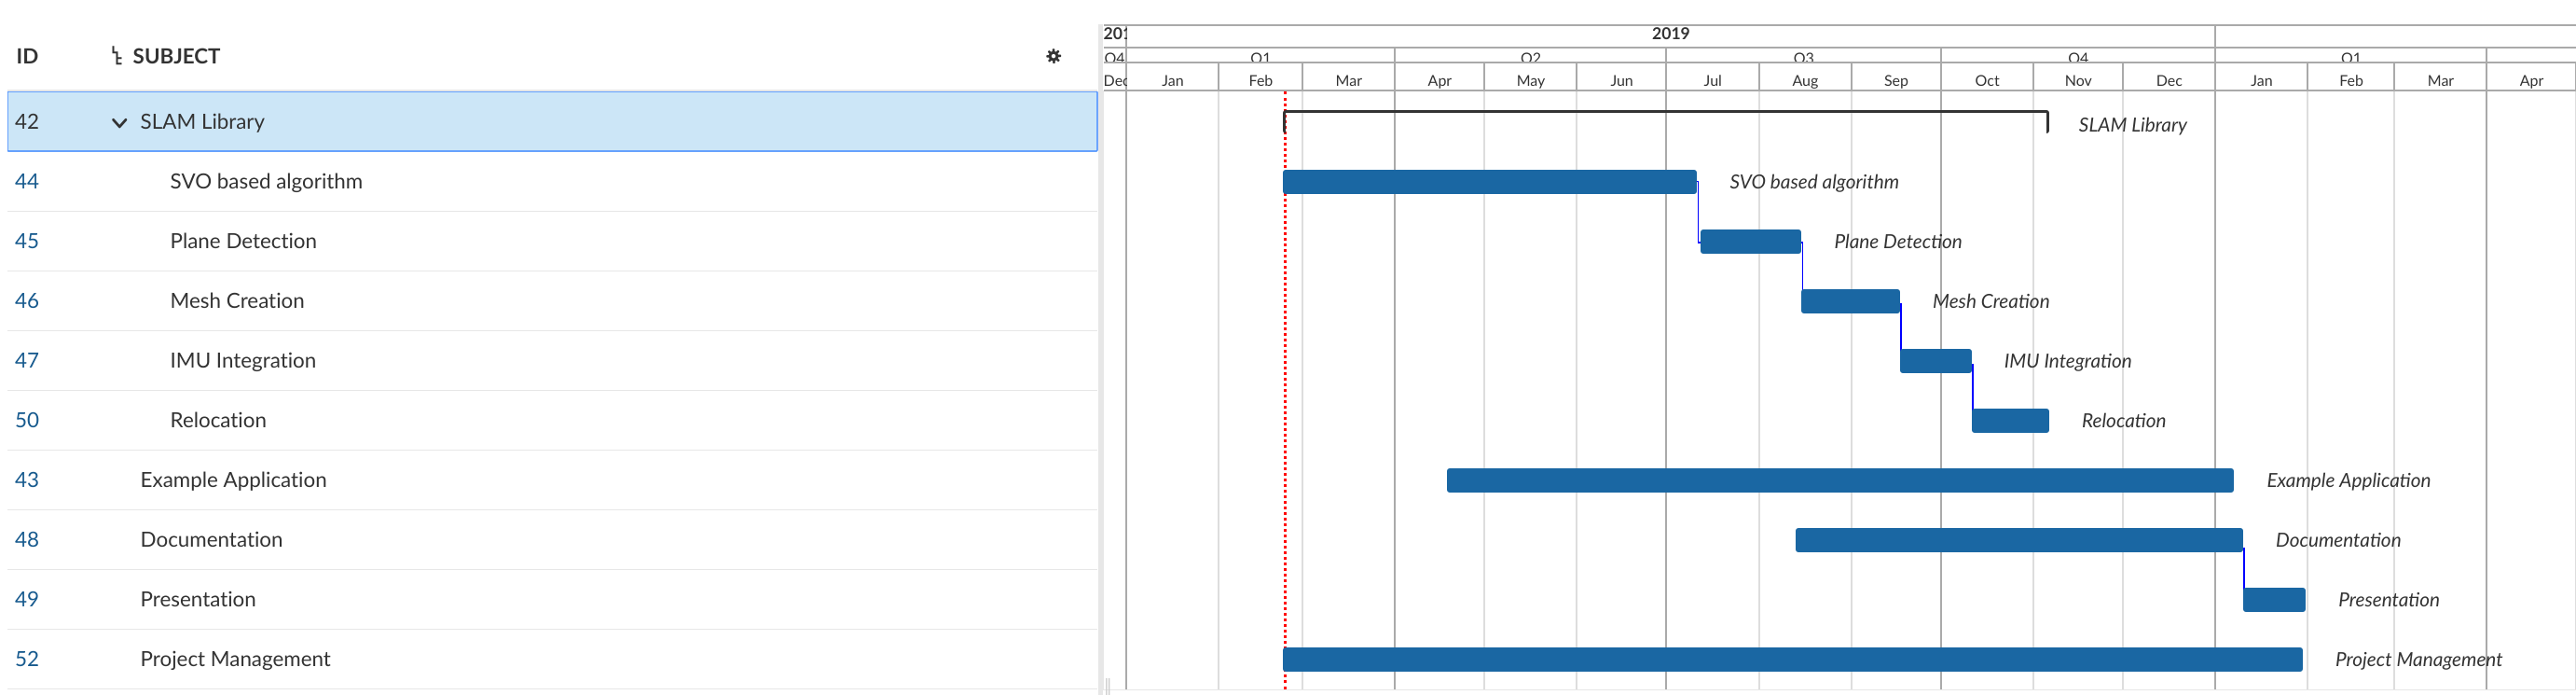
\includegraphics[width=1.0\textwidth]{img/gantt.png}
	\caption{Initial planing}\label{fig:gantt}
\end{figure}

\chapter{Algorithm}
In this chapter we analyse an algorithm that can be used to solve the SLAM problem.

\section{ORB SLAM}

\section{SVO SLAM}
While ORB SLAM is well documented and can do loop closing, it is difficult to optimize the algorithm for realtime applications.

\subsection{Initialization}\label{sec:initialization}
In this project we use a stereo camera therefore the initialization step is simpler than in the monocular case. The algorithm performs the following steps.
\begin{enumerate}
	\item{Search FAST keypoints on the whole image}
	\item{Do Sobel filtering in horizontal direction}
	\item{Divide image in 16x16 blocks}
	\item{Select one FAST corner in each block}
		\subitem{If no FAST corner can be found, use point with highest gradient as keypoint}
	\item{Calculate depth fore each keypoint}
		\subitem{Find the smallest intensity difference along the epipolar line}
		\subitem{The difference between these two points is the disparity (1/depth)}
\end{enumerate}

This step is described in \cite{svo2} section IX.A. We use a multi camera approach. We need to do the initialization step when we get the first frame as well as when we insert a new keyframe.

\subsection{Sparse Image Alignment}\label{sec:sia}

From the initialization step we optain a initial point cloud. We use this point cloud to estimate the pose and motion of the camera. We try to find a Pose that minimizes the photometric error of small patches around the keypoints found in section \ref{sec:initialization}. We do that by minimizing the formula shown in equation \ref{eq:intensity}. We use equation \ref{eq:cm} to project the 3D point cloud to the current frame. By using Levenberg-Marquardt we can minimize the intensity difference by changing the values of the extrinsic matrix $r_{ij}$ and $t_{x,y,z}$. As initial guess for the pose we use the current pose and add the motion model. The motion model is the difference between the pose in the previous frame ($t-1$) and frame $t-2$.

\begin{equation}\label{eq:intensity}
	I_{TD}=\sum_{i=0}^{i=N}I_{F-1}(x_{F-1,i},y_{F-1,i})-I_{F}(x_{F,i},y_{F,i})
\end{equation}
Where:
\begin{align*}
	I_{TD} &:					\text{Total intensity difference over all keypoints}\\
	I_{F-1} &:				\text{Previous grayscale image}\\
	I_{F} &:					\text{Current grayscale image}\\
	x_{KF},y_{KF} &:	\text{x,y position in keyframe}\\
	N &:							\text{Total number of keypoints}\\
	x_{F},y_{F} &:		\text{x,y posiiton in current frame}
\end{align*}

\begin{equation}\label{eq:cm}
  \begin{pmatrix}
		f_x & \gamma & c_x \\
		0 & f_y & c_y \\
		0 & 0 & 1 \\
	\end{pmatrix}*
	\begin{pmatrix}
		r_{11} & r_{12} & r_{13} & t_x \\
		r_{21} & r_{22} & r_{23} & t_y \\
		r_{31} & r_{32} & r_{33} & t_z \\
	\end{pmatrix}
	\begin{pmatrix}
		X \\
		Y \\
		Z \\
		1
	\end{pmatrix}=
	\begin{pmatrix}
		u \\
		v \\
		s
  \end{pmatrix}
\end{equation}
\begin{equation}\label{eq:cm_normalized}
	\begin{pmatrix}
		x \\
		y
	\end{pmatrix}=
	\begin{pmatrix}
		u/s \\
		v/s 
  \end{pmatrix}
\end{equation}
Where:
\begin{align*}
  X,Y,Z			&: \text{point in the 3D world}\\
	u,v,s	   	&: \text{point in 2D image not normalize}\\
	x,y				&: \text{point in 2D image normalized with s}\\
	f_x,f_y  	&: \text{focal length of the camera}\\
  c_x,c_y  	&: \text{principal point}\\
  t_x,t_y,t_z	&: \text{location of the camera}\\
  r_{ij}	&: \text{part of the rotation matrix}
\end{align*}

This step is described in \cite{svo2} in section IV.A. We get a first estimate for the pose. However, because we estimate the current pose by using the previous frame we will get a drift in the long term. Therefore, we need to refine the pose by using the keyframe as reference.\\
If less than 80\% of the keypoints are trackable we need to insert a new keyframe based on the previous frame. In comparison SVO inserts a new keyframe if the movement is more than 12\% of the average depth. In a first step we try to do it as described, however maybe this needs to change in the future. See \cite{svo2} section X.D for the implementation details.

\subsection{Refinement}\label{sec:refinement}

The refinement step is necessary to reduce the drift over time by taking the information of the keyframe into account. We use the Lucas-Kanade algorithm to find an Affine transformation Matrix that minimizes the photometric error between all keypoints of the keyframe and the current frame. This will give us a reprojection error. We try to minimize this reprojection error by do ing a bundle adjustment over the pose (motion only) and over the 3D point cloud (structure only).\\

Lucas-Kanade tries to find the movement of points by trying to find a movement (dx, dy) that minimizes the intensity difference as shown in equation \ref{eq:lucaskanade}
\begin{equation}\label{eq:lucaskanade}
	I(x,y,t)=I(x+dx, y+dy, t+dt)
\end{equation}
Where:
\begin{align*}
	I(x,y,t)						&:	\text{intensity in template}\\
	I(x+dx, y+dy, t+dt) &:	\text{intensity in new image t+dt, moved by dx and dy}
\end{align*}

Lucas Kanade tries to solve this equation by assuming that the intensity gradient at a keypoint will point in the direction of the movement \cite{lucas_kanade}. The SVO paper doesn't use Lucas Kanade to do the 2d point adjustment. They use the Inverse Compositional method instead. In comparison to Lucas Kanade they will find one Affine Warp matrix that describes the movement of all points. Lucas Kanade as implemented in OpenCV will move each point separate. However, because no Inverse Compositional method is available in OpenCV Lucas Kanade was used as a first implementation. This will be less efficient than using the Inverse Compositional method.

\subsubsection{Pose refinement}
In section \ref{sec:sia} we estimated the pose of the current frame by using the 3D point cloud and the previous image. Based on the estimated pose we then refined the 2D point position as described in section \ref{sec:refinement}. Now we need to update the estimated pose in regards to the new 2D point position. This is done by minimizing the reprojection error when changing the pose. We use Levenberg-Marquardt to minimize the pose in this step.
\begin{equation}\label{eq:pose_refinement}
	min((x - x')^2 + (y -y')^2)
\end{equation}
Where:
\begin{align*}
	x,y		&: \text{x,y position in image after refinement}\\
	x',y' &: \text{x,y reprojection of 3D point by using \ref{eq:cm}}
\end{align*}

\subsection{Finding gradient for optimization}
To speed up the optimization a predefined gradient can be calculated. The method to find such a gradient is related to the Lucas-Kanade optical flow method. Instead of searching a Warp matrix we search a transformation matrix in this scenario. We have two images $I_{k-1}$ and $I_{k}$. We know the pose of image k-1 $T_{k-1}$ . We search the pose $T_k$.\\
While the inverse compositional Lucas Kanade algorithm tries to find the optimal Warp matrix. We try to find the optimal pose.
\subsubsection{Lucas Kanade Algorithm}
Lets assume we have a warp matrix in the following form:
\begin{equation}\label{eq:lk_warp}
	p=\begin{pmatrix}
		p_{11} & p_{12} & p_{13} \\
		p_{21} & p_{22} & p_{23}
	\end{pmatrix}
\end{equation}
\begin{align*}
	p				&:	\text{warp matrix}\\
	p_{ij}	&:	\text{parameter of warp matrix}
\end{align*}


Lucas Kanade tries to optimize the following problem \cite{inverse_compositional}:
\begin{equation}\label{eq:lk_problem}
	\sum_x\sum_y(I_{k}(x',x')-I_{k-1}(x,y))^2
\end{equation}
\begin{align*}
	x,y				&:	\text{Pixel position in template}\\
	x',y'			&:	\text{Pixel position in current image}\\
	I_{k-1}		&:	\text{Template image}\\
	I_{k}			&:	\text{Current image}
\end{align*}

\begin{equation}
	W=
	\begin{pmatrix}
		x' \\
		y'
	\end{pmatrix}=
	\begin{pmatrix}
		p_{11} & p_{12} & p_{13} \\
		p_{21} & p_{22} & p_{23}
	\end{pmatrix}*
	\begin{pmatrix}
		x\\
		y\\
		1
	\end{pmatrix}=
	\begin{pmatrix}
		p_{11}*x + p_{12}*y + p_{13} \\
		p_{21}*x + p_{22}*y + p_{23}
	\end{pmatrix}
\end{equation}
\begin{align*}
	W					&:	\text{Warp}\\
	x',y'			&:	\text{Pixel position in current image}\\
	x,y				&:	\text{Pixel position in template}\\
	p_{ij}		&:	\text{parameter of warp matrix}
\end{align*}

Because \ref{eq:lk_problem} is a nonlinear problem we have to solve it with a nonlinear solver (e.g. Gauss-Newton or Gradient Descent). The problem is solved by iteratively changing the Warpmatrix in the direction of a gradient until the difference of the intensities are minimal:
\begin{equation}
	\begin{pmatrix}
		x' \\
		y'
	\end{pmatrix}=
	\begin{pmatrix}
		p_{11}+\Delta p_{11} & p_{12}+\Delta p_{12} & p_{13}+\Delta p_{13} \\
		p_{21}+\Delta p_{21} & p_{22}+\Delta p_{22} & p_{23}+\Delta p_{23}
	\end{pmatrix}*
	\begin{pmatrix}
		x\\
		y\\
		1
	\end{pmatrix}
\end{equation}
\begin{align*}
	x',y'					&:	\text{Pixel position in current image}\\
	x,y						&:	\text{Pixel position in template}\\
	p_{ij}				&:	\text{parameter of warp matrix}\\
	\Delta p_{ij}	&:	\text{change of $p_{ij}$ per iteration}
\end{align*}


After each iteration we set $p=p_{i-1}+\Delta p$.\\
We can solve this problem by approximating the gradient. However it would slow down the calculation. Therefore, Lucas Kanade calculates the gradient by doing a first order Taylor approximation of the problem:
\begin{equation}\label{eq:lk_taylor}
	\sum_x\sum_y(I_{k}(x_{i-1}',y_{i-1}')+\nabla I_{k}*\frac{\sigma W}{\sigma p}*\Delta p-I_{k-1}(x,y))^2
\end{equation}
\begin{align*}
	x,y				&:	\text{Pixel position in template}\\
	x',y'			&:	\text{Pixel position in current image}\\
	I_{k-1}		&:	\text{Template image}\\
	I_{k}			&:	\text{Current image}\\
	\nabla I	&:	\text{Gradient in image I at position x',y'}
\end{align*}
We want to find $\Delta p$ which is our gradient. To make this work we have to derive equation \ref{eq:lk_taylor}. This gives us:
\begin{equation}
	2*\sum_x\sum_y\begin{bmatrix}\nabla I_{k}*\frac{\sigma W}{\sigma p}\end{bmatrix}^T*\begin{bmatrix}I_{k}(x_{i-1}',y_{i-1}')+\nabla I_{k}*\frac{\sigma W}{\sigma p}*\Delta p-I_{k-1}(x,y)\end{bmatrix}
\end{equation}
We can now find $\Delta p$ by moving it to the left:
\begin{equation}\label{eq:lk_dp}
	\Delta p=(\sum_x\sum_y\begin{bmatrix}\nabla I_{k}*\frac{\sigma W}{\sigma p}\end{bmatrix}^T*\begin{bmatrix}\nabla I_{k}*\frac{\sigma W}{\sigma p}\end{bmatrix})^{-1}
	*\sum_x\sum_y\begin{bmatrix}\nabla I_{k}*\frac{\sigma W}{\sigma p}\end{bmatrix}^T*\begin{bmatrix}I_{k-1}(x,y) - I_{k}(x_{i-1}',y_{i-1}'\end{bmatrix}
\end{equation}

$\frac{\sigma W}{\sigma p}$ is the Jacobian matrix and looks as follows:
\begin{equation}
	\frac{\sigma W}{\sigma p}=
	\begin{pmatrix}
		x & y & 1 & 0 & 0 & 0 \\
		0 & 0 & 0 & x & y & 1
	\end{pmatrix}
\end{equation}

All parameters in equation \ref{eq:lk_dp} are known and can be calculated for a given x,y and p. However, the following part of equation \ref{eq:lk_dp} is time consuming to calculate and has to be inverted:
\begin{equation}
	\Delta H=(\sum_x\sum_y\begin{bmatrix}\nabla I_{k}*\frac{\sigma W}{\sigma p}\end{bmatrix}^T*\begin{bmatrix}\nabla I_{k}*\frac{\sigma W}{\sigma p}\end{bmatrix})
\end{equation}
H is called the Hessian matrix. Unfortunately we need to calculate this matrix in each iteration. The inverse compositional Lucas Kanade algorithm tries to solve this problem by wrapping the template to the current image instead of the current image to the template.

\subsection{Inverse compositional Lucas Kanade}

The inverse compositional Lucase Kanade algorithm does more or less the same as the normal Lucas Kanade algorithm but it searches the inverse wrap update at each iteration. The problem basically stays the same but we switch the role of the template with the one of the image which first doesn't have any effect:
\begin{equation}\label{eq:iclk_problem}
	\sum_x\sum_y(I_{k-1}(x'',y'')-I_{k}(x',y'))^2
\end{equation}
\begin{align*}
	x'',y''		&:	\text{Warped pixel position in the template}\\
	x',y'			&:	\text{Pixel position in the current image}\\
	I_{k-1}		&:	\text{Template image}\\
	I_{k}			&:	\text{Current image}
\end{align*}

What is different this time is that we wrap the template with $\Delta p$:
\begin{equation}
	\begin{pmatrix}
		x'' \\
		y''
	\end{pmatrix}=
	\begin{pmatrix}
		\Delta p_{11} & \Delta p_{12} & \Delta p_{13} \\
		\Delta p_{21} & \Delta p_{22} & \Delta p_{23}
	\end{pmatrix}*
	\begin{pmatrix}
		x\\
		y\\
		1
	\end{pmatrix}
\end{equation}
\begin{align*}
	x,y						&:	\text{Original pixel position in template}\\
	x'',y''				&:	\text{Warped pixel position in template}\\
	\Delta p_{ij}	&:	\text{change of $p_{ij}$ per iteration}
\end{align*}

\begin{equation}
	\begin{pmatrix}
		x' \\
		y'
	\end{pmatrix}=
	\begin{pmatrix}
		p_{11} & p_{12} & p_{13} \\
		p_{21} & p_{22} & p_{23}
	\end{pmatrix}*
	\begin{pmatrix}
		x\\
		y\\
		1
	\end{pmatrix}
\end{equation}
\begin{align*}
	x',y'					&:	\text{Pixel position in current image}\\
	x,y						&:	\text{Original pixel position in template}\\
	p_{ij}				&:	\text{parameter of warp matrix}\\
\end{align*}

With this we separate the update step from the wrapping of the image. The update step will then be $p=p_{i-1}+(\Delta p)^{-1}$. If we do the first order taylor approximation again we get:

\begin{equation}\label{eq:iclk_taylor}
	\sum_x\sum_y(I_{k-1}(x,y)+\nabla I_{k-1}*\frac{\sigma W}{\sigma p}*\Delta p-I_{k}(x',y'))^2
\end{equation}
\begin{align*}
	x,y				&:	\text{Original pixel position in template}\\
	x',y'			&:	\text{Pixel position in current image}\\
	I_{k-1}		&:	\text{Template image}\\
	I_{k}			&:	\text{Current image}\\
	\nabla I	&:	\text{Gradient in image I at position x',y'}
\end{align*}

This gives us for $\Delta p$:
\begin{equation}\label{eq:iclk_dp}
	\Delta p=(\sum_x\sum_y\begin{bmatrix}\nabla I_{k-1}*\frac{\sigma W}{\sigma p}\end{bmatrix}^T*\begin{bmatrix}\nabla I_{k-1}*\frac{\sigma W}{\sigma p}\end{bmatrix})^{-1}
	*\sum_x\sum_y\begin{bmatrix}\nabla I_{k-1}*\frac{\sigma W}{\sigma p}\end{bmatrix}^T*\begin{bmatrix}I_{k}(x_{i-1}',y_{i-1}') - I_{k-1}(x,y)\end{bmatrix}
\end{equation}

Compared to the normal Lucas-Kanade algorithm the Hessian Matrix H is now constant for all iterations and we don't have to do the expensive calculation at every iteration:
\begin{equation}
	\Delta H=\sum_x\sum_y\begin{bmatrix}\nabla I_{k-1}*\frac{\sigma W}{\sigma p}\end{bmatrix}^T*\begin{bmatrix}\nabla I_{k-1}*\frac{\sigma W}{\sigma p}\end{bmatrix}
\end{equation}

Because we only have to calculate the Hessian matrix once, the inverse computational Lucas Kanade is more efficient then the Lucas Kanade algorithm.

\subsubsection{3D cloud refinement}
After refining the pose we still have a small reprojection error. We can try to minimize this error by adjusting the 3D position for each point. Here we do the same thing as in equation \ref{eq:pose_refinement} but we now change the 3D point position instead of the pose. Because we need to do that for all point this is more computational expensive than the previous step. Instead of Levenberg-Marquardt we use normal Gradient-Descent in this step, because the here described problem is an underdeterminated problem. However, we can still find a local minimum. This step follows section V.B in \cite{svo2}. However, pose and 3D cloud is only updated for the last camera frame. We do not bundle adjust the whole trajectory.

\subsection{Mapping}

Mapping can be solved in a separate thread. The mapping thread decides if a new keyframe must be insert. If no keyframe is required, we can use the current frame to update the depth of the 3D cloud by adjusting the inverse depth with a Kalman Filter. Mapping is not solved yet.

\begin{thebibliography}{1}

	\bibitem{svo}
	Christian Forster et al\\
	\textit{SVO: Semi-Direct Visual Odometry for Monocular and Multi-Camera Systems}\\
	doi:10.1109/TRO.2016.2623335

	\bibitem{svo2}
	Christian Forster et al\\
	\textit{SVO: Semi-Direct Visual Odometry for Monocular and Multi-Camera Systems}\\
	doi:10.1109/TRO.2016.2623335

	\bibitem{lucas_kandae}
	OpenCV\\
	\textit{Optical Flow}\\
	https://docs.opencv.org/4.0.1/d7/d8b/tutorial\_py\_lucas\_kanade.html


	\bibitem{inverse_compositional}
	S. Baker and I. Matthews\\
	\textit{Lucas-kanade 20 years on: A unifying framework}
	Int. J. Comput. Vis., 56(3):221–255, 2004.


\end{thebibliography}

\end{document}
